\documentclass{beamer}
\usepackage[utf8]{inputenc}
\usepackage{graphicx, epsfig}
\usepackage{amsmath,mathrsfs,amsfonts,amssymb}
\usepackage{floatflt}
\usepackage{epic,ecltree}
\usepackage{mathtext}
\usepackage{fancybox}
\usepackage{fancyhdr}
\usepackage{multirow}
\usepackage{enumerate}
\usepackage{epstopdf}
\usepackage{multicol}
\usepackage{algorithm}
\usepackage[noend]{algorithmic}
\usepackage{tikz}
\usepackage{blindtext}
\usetheme{default}%{Singapore}%{Warsaw}%{Warsaw}%{Darmstadt}
\usecolortheme{default}

\setbeamerfont{title}{size=\Huge}
\setbeamertemplate{footline}[page number]{}

\setbeamertemplate{section in toc}[sections numbered]


\makeatletter
\newcommand\HUGE{\@setfontsize\Huge{35}{40}}
\makeatother    

\setbeamerfont{title}{size=\HUGE}
\beamertemplatenavigationsymbolsempty

% latin bold lower
\newcommand{\ba}{\mathbf{a}} 
\newcommand{\bc}{\mathbf{c}} 
\newcommand{\be}{\mathbf{e}} 
\newcommand{\bh}{\mathbf{h}} 
\newcommand{\bp}{\mathbf{p}} 
\newcommand{\bt}{\mathbf{t}} 
\newcommand{\bs}{\mathbf{s}} 
\newcommand{\bu}{\mathbf{u}} 
\newcommand{\bv}{\mathbf{v}} 
\newcommand{\bw}{\mathbf{w}} 
\newcommand{\bx}{\mathbf{x}} 
\newcommand{\by}{\mathbf{y}} 
\newcommand{\bz}{\mathbf{z}} 

% latin bold upper
\newcommand{\bA}{\mathbf{A}} 
\newcommand{\bB}{\mathbf{B}} 
\newcommand{\bC}{\mathbf{C}} 
\newcommand{\bI}{\mathbf{I}} 
\newcommand{\bJ}{\mathbf{J}} 
\newcommand{\bL}{\mathbf{L}} 
\newcommand{\bM}{\mathbf{M}} 
\newcommand{\bP}{\mathbf{P}}
\newcommand{\bQ}{\mathbf{Q}} 
\newcommand{\bR}{\mathbf{R}} 
\newcommand{\bT}{\mathbf{T}} 
\newcommand{\bU}{\mathbf{U}} 
\newcommand{\bV}{\mathbf{V}} 
\newcommand{\bW}{\mathbf{W}} 
\newcommand{\bX}{\mathbf{X}} 
\newcommand{\bY}{\mathbf{Y}} 
\newcommand{\bZ}{\mathbf{Z}} 

% latin cal upper
\newcommand{\cF}{\mathcal{F}} 
\newcommand{\cG}{\mathcal{G}} 
\newcommand{\cI}{\mathcal{I}} 
\newcommand{\cL}{\mathcal{L}} 
\newcommand{\cM}{\mathcal{M}} 
\newcommand{\cN}{\mathcal{N}} 
\newcommand{\cP}{\mathcal{P}} 
\newcommand{\cS}{\mathcal{S}} 
\newcommand{\cT}{\mathcal{T}} 
\newcommand{\cW}{\mathcal{W}} 
\newcommand{\cX}{\mathcal{X}} 
\newcommand{\cZ}{\mathcal{Z}} 

% latin bb upper
\newcommand{\bbE}{\mathbb{E}} 
\newcommand{\bbI}{\mathbb{I}} 
\newcommand{\bbP}{\mathbb{P}} 
\newcommand{\bbR}{\mathbb{R}} 

% greek bold lower
\newcommand{\bepsilon}{\boldsymbol{\epsilon}} 
\newcommand{\btheta}{\boldsymbol{\theta}} 
\newcommand{\blambda}{\boldsymbol{\lambda}} 
\newcommand{\bpi}{\boldsymbol{\pi}} 
\newcommand{\bmu}{\boldsymbol{\mu}} 
\newcommand{\bsigma}{\boldsymbol{\sigma}} 
\newcommand{\bphi}{\boldsymbol{\phi}} 

% greek bold upper
\newcommand{\bSigma}{\boldsymbol{\Sigma}} 

\DeclareMathOperator*{\argmin}{arg\,min}
\DeclareMathOperator*{\argmax}{arg\,max}

\newcommand{\createdgmtitle}[1]{\title[\hbox to 56mm{Deep Generative Models  \hfill\insertframenumber\,/\,\inserttotalframenumber}]
	{\vspace{1cm} \\ \textbf{Deep Generative Models} \\ {\Huge Lecture #1}}
	\author{Roman Isachenko}
		\institute{
\includegraphics[width=0.7cm]{../utils/aimasterslogo} \LARGE{AI Masters}}
	\date{2024, Spring}
}

\usepackage{tikz}
\usetikzlibrary{arrows,shapes,positioning,shadows,trees}

\newcommand\myfootnote[1]{%
  \tikz[remember picture,overlay]
  \draw (current page.south west) +(1in + \oddsidemargin,0.5em)
  node[anchor=south west,inner sep=0pt]{\parbox{\textwidth}{%
      \rlap{\rule{10em}{0.4pt}}\raggedright\scriptsize \textit{#1}}};}

\newcommand\myfootnotewithlink[2]{%
  \tikz[remember picture,overlay]
  \draw (current page.south west) +(1in + \oddsidemargin,0.5em)
  node[anchor=south west,inner sep=0pt]{\parbox{\textwidth}{%
      \rlap{\rule{10em}{0.4pt}}\raggedright\scriptsize\href{#1}{\textit{#2}}}};}
      
\AtBeginSection[]
      {
      	\begin{frame}{Outline}
      		\tableofcontents[currentsection]
      	\end{frame}
      }
      \AtBeginSubsection[]{
      	\begin{frame}{Outline}
      		\tableofcontents[currentsection,currentsubsection]
      	\end{frame}
}
\createdgmtitle{9}
%--------------------------------------------------------------------------------
\begin{document}
%--------------------------------------------------------------------------------
\begin{frame}[noframenumbering,plain]
%\thispagestyle{empty}
\titlepage
\end{frame}
%=======
\begin{frame}{Recap of previous lecture}
	\begin{block}{WGAN objective}
		\vspace{-0.5cm}
		\[
		\min_{\btheta} W(\pi || p) = \min_{\btheta} \max_{\bphi \in \boldsymbol{\Phi}} \left[ \bbE_{\pi(\bx)} f_{\bphi}(\bx)  - \bbE_{p(\bz)} f_{\bphi}(G_{\btheta}(\bz))\right].
		\]
		\vspace{-0.5cm}
	\end{block}
	\begin{itemize}
		\item Function~$f$ in WGAN is usually called $\textit{critic}$.
		\item If parameters $\bphi$ lie in a compact set $\boldsymbol{\Phi} \in [-c, c]^d$ then $f(\bx, \bphi)$ will be $K$-Lipschitz continuous function. 
	\end{itemize}
	\begin{multline*}
		K \cdot W(\pi || p) = \max_{\| f \|_L \leq K} \left[ \bbE_{\pi(\bx)} f(\bx)  - \bbE_{p(\bx)} f(\bx)\right] \geq \\  \geq \max_{\bphi \in \boldsymbol{\Phi}} \left[ \bbE_{\pi(\bx)} f_{\bphi}(\bx)  - \bbE_{p(\bx)} f_{\bphi}(\bx)\right]
	\end{multline*}
	\textit{"Weight clipping is a clearly terrible way to enforce a Lipschitz constraint"}
	\myfootnotewithlink{https://arxiv.org/abs/1701.07875}{Arjovsky M., Chintala S., Bottou L. Wasserstein GAN, 2017}
\end{frame}
%=======
\begin{frame}{Recap of previous lecture}
	\begin{block}{Theorem}
		Let $\pi(\bx)$ and $p(\bx)$ be two distribution in $\cX$, a compact metric space. Let $\gamma$ be the optimal transportation plan between $\pi(\bx)$ and $p(\bx)$. Then
		\vspace{-0.4cm}
		\[
			\bbP_{(\by, \bz) \sim \gamma} \left[ \nabla f^*(\hat{\bx}_t) = \frac{\bz - \hat{\bx}_t}{\| \bz - \hat{\bx}_t \|} \right] = 1.
		\]
		\vspace{-0.6cm}
	\end{block}
	\begin{block}{Gradient penalty}
		\vspace{-0.5cm}
		\[
			W(\pi || p) = \underbrace{\bbE_{\pi(\bx)} f(\bx)  - \bbE_{p(\bx)} f(\bx)}_{\text{original critic loss}} + \lambda \underbrace{\bbE_{U[0, 1]} \left[ \left( \| \nabla f(\hat{\bx}) \|_2 - 1 \right) ^ 2\right]}_{\text{gradient penalty}}.
		\]
		\vspace{-0.5cm}
	\end{block}
	Samples $\hat{\bx}_t = t \by + (1 - t) \bz$ with $t \in [0, 1]$ are uniformly sampled along straight lines between pairs of points: $\by$ from the data distribution $\pi(\bx)$ and $\bz$ from the generator distribution $p(\bx | \btheta)$.
	\myfootnote{
	\href{https://arxiv.org/abs/1701.07875}{Arjovsky M., Chintala S., Bottou L. Wasserstein GAN, 2017} \\
	\href{https://arxiv.org/abs/1704.00028}{Gulrajani I. et al. Improved Training of Wasserstein GANs, 2017} }
\end{frame}
%=======
\begin{frame}{Recap of previous lecture}
	\vspace{-0.3cm}
	\begin{block}{f-divergence minimization}
		\vspace{-0.3cm}
		\[
			D_f(\pi || p) = \bbE_{p(\bx)}  f\left( \frac{\pi(\bx)}{p(\bx)} \right) \rightarrow \min_p.
		\]
		Here $f: \bbR_+ \rightarrow \bbR$ is a convex, lower semicontinuous function satisfying $f(1) = 0$.
	\end{block}
	\begin{block}{Variational divergence estimation}
		\vspace{-0.3cm}
		\[
			D_f(\pi || p) \geq \sup_{T \in \cT} \left[\bbE_{\pi}T(\bx) -  \bbE_p f^*(T(\bx)) \right],
		\]
		\vspace{-0.7cm}
	\end{block}
	\begin{block}{Fenchel conjugate}
		\vspace{-0.7cm}
		\[
		f^*(t) = \sup_{u \in \text{dom}_f} \left( ut - f(u) \right), \quad f(u) = \sup_{t \in \text{dom}_{f^*}} \left( ut - f^*(t) \right)
		\]
		\vspace{-0.5cm}
	\end{block}
	\textbf{Note:} To evaluate lower bound we only need samples from $\pi(\bx)$ and $p(\bx)$. Hence, we could fit implicit generative model.
	\myfootnotewithlink{https://arxiv.org/abs/1606.00709}{Nowozin S., Cseke B., Tomioka R. f-GAN: Training Generative Neural Samplers using Variational Divergence Minimization, 2016}
\end{frame}
%=======
\begin{frame}{Recap of previous lecture}
	How to evaluate likelihood-free models?
	
	$p(y | \bx)$ -- pretrained image classification model (e.g. ImageNet classifier).
	\begin{block}{What do we want from samples?}
		\begin{itemize}
			\item \textbf{Sharpness}
			\begin{figure}
				\centering
				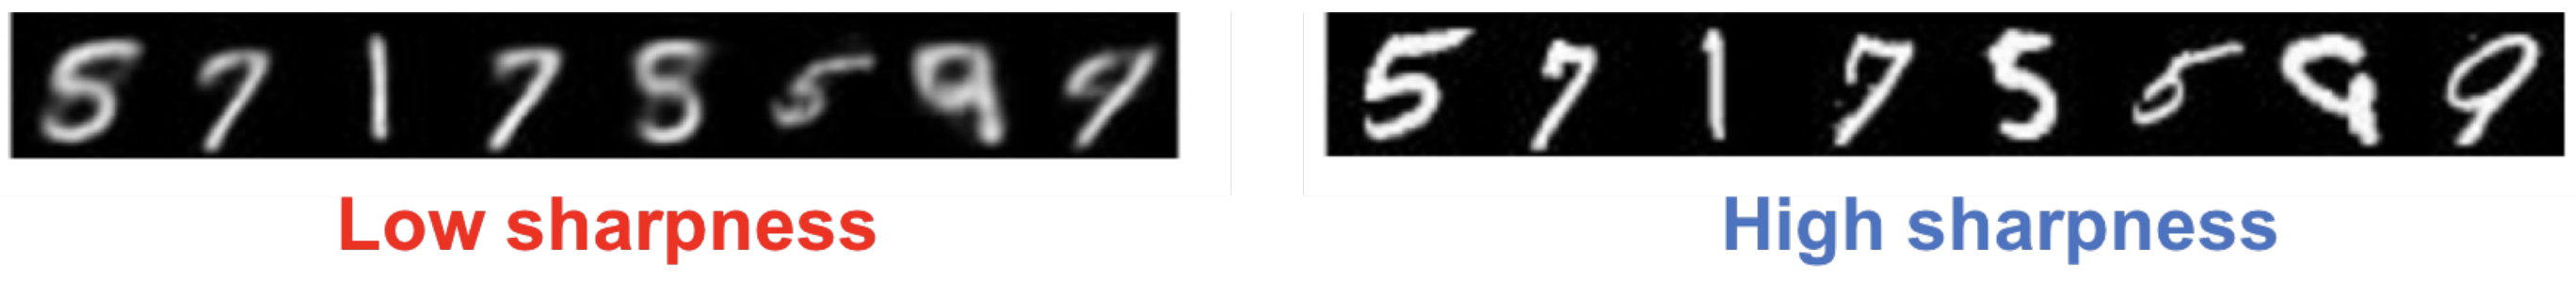
\includegraphics[width=0.9\linewidth]{figs/sharpness}
			\end{figure}
			$p(y | \bx)$ has low entropy (each image $\bx$ should have distinctly recognizable object).
			\item \textbf{Diversity}
			\begin{figure}
				\centering
				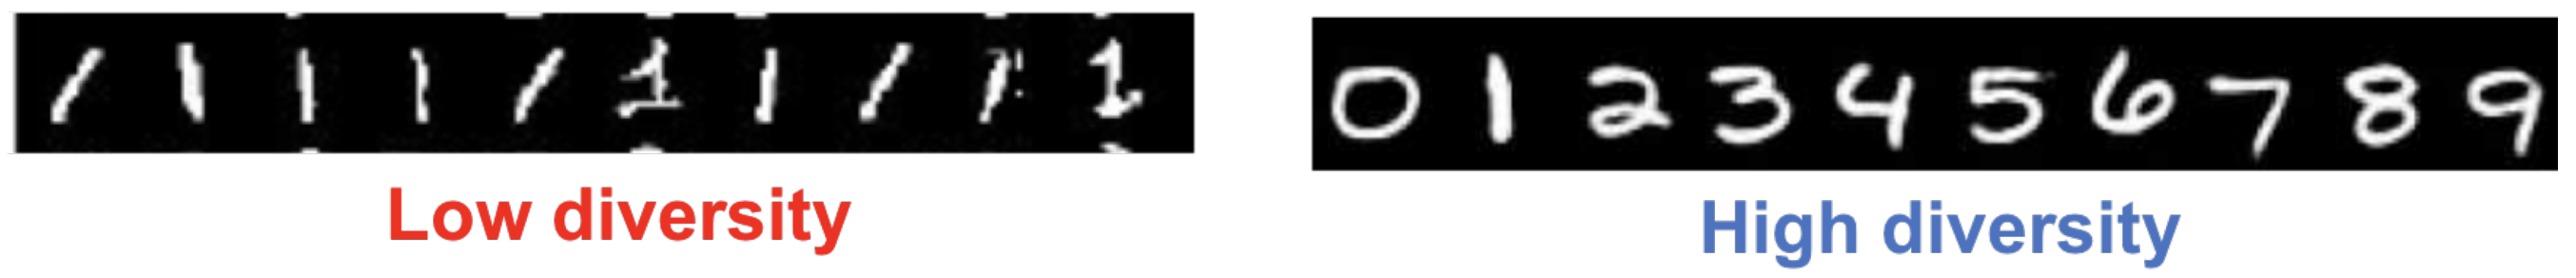
\includegraphics[width=0.9\linewidth]{figs/diversity}
			\end{figure}
			$p(y) = \int p(y | \bx) p(\bx) d \bx$ has high entropy (there should be as many classes generated as possible).
		\end{itemize}
	\end{block}
	\myfootnotewithlink{https://deepgenerativemodels.github.io}{image credit: https://deepgenerativemodels.github.io}
\end{frame}
%=======
\begin{frame}{Outline}
	\tableofcontents
\end{frame}
%=======
\section{Evaluation of likelihood-free models}
%=======
\subsection{Maximum Mean Discrepancy (MMD)}
%=======
\begin{frame}{Maximum Mean Discrepancy (MMD)}
	\begin{block}{Theorem}
		$\pi(\bx) = p(\by)$ if and only if $\bbE_{\pi(\bx)} f(\bx) = \bbE_{p(\by)} f(\by)$ for any bounded and continuous $f$.
	\end{block}
	\vspace{-0.3cm}
	\[
		\text{MMD}(\pi, p) = \sup_f \left[ \bbE_{\pi(\bx)} f(\bx) - \bbE_{p(\bx)} f(\bx) \right]
	\]	
	\vspace{-0.3cm}
	\begin{block}{Theorem (Reproducing Kernel Hilbert Space)}
		\vspace{-0.6cm}
		\[
			\text{MMD}^2(\pi, p) = \bbE_{(\bx, \bx')} k(\bx, \bx') + \bbE_{(\by, \by')} k(\by, \by') - 2 \bbE_{(\bx, \by)} k(\bx, \by),
		\]
		Here 
		\begin{itemize}
			\item $k(\bx, \by)$ is a positive definite, symmetric kernel function (for example $k(\bx, \by) = \frac{\exp(\|\bx - \by\|^2)}{\sigma^2}$);
			\item $f(\bx) = \langle f, \phi(\bx) \rangle_{\mathcal{H}}$;
			\item $\phi(\bx) = k(\cdot, \bx)$.
		\end{itemize} 
		\vspace{-0.3cm}
	\end{block}
	\myfootnotewithlink{https://arxiv.org/abs/2401.09603}{Jayasumana S. et al. Rethinking FID: Towards a Better Evaluation Metric for Image Generation, 2024}
\end{frame}
%=======
\begin{frame}{Maximum Mean Discrepancy (MMD)}
		\vspace{-0.6cm}
		\[
			\text{MMD}^2(\pi, p) = \bbE_{(\bx, \bx')} k(\bx, \bx') + \bbE_{(\by, \by')} k(\by, \by') - 2 \bbE_{(\bx, \by)} k(\bx, \by),
		\]
		\vspace{-0.3cm}
	\begin{figure}
		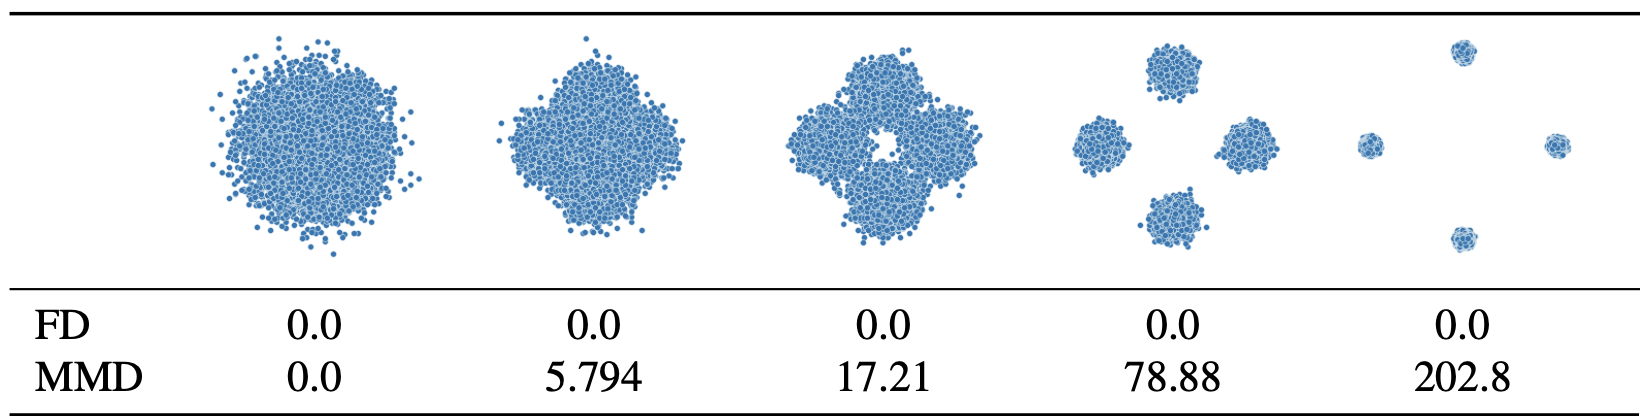
\includegraphics[width=0.95\linewidth]{figs/mmd_normal}
	\end{figure}
	\begin{itemize}
		\item Needs less sample size for evaluation.
		\item High dependence on the pretrained classification model.
		\item Works with any distribution!
	\end{itemize}
	\myfootnotewithlink{https://arxiv.org/abs/2401.09603}{Jayasumana S. et al. Rethinking FID: Towards a Better Evaluation Metric for Image Generation, 2024}
\end{frame}
%=======
\subsection{Precision-Recall}
%=======
\begin{frame}{Precision-Recall}
	\begin{block}{What do we want from samples}
		\begin{itemize}
			\item \textbf{Sharpness}: generated samples should be of high quality.
			\item \textbf{Diversity}: their variation should match that observed in the training set.
		\end{itemize}
	\end{block}
	\vspace{-0.5cm}
	\begin{figure}
		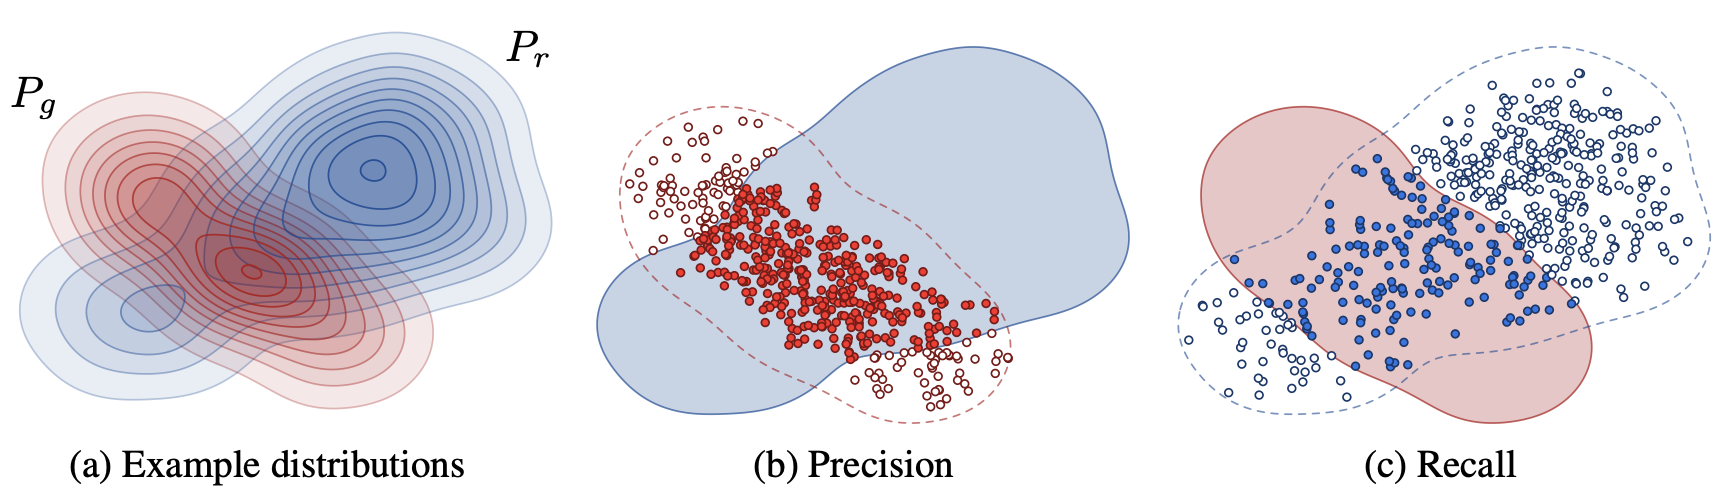
\includegraphics[width=0.95\linewidth]{figs/pr_curve}
	\end{figure}
	\vspace{-0.3cm}
	\begin{itemize}
		\item \textbf{Precision} denotes the fraction of generated images that are realistic.
		\item \textbf{Recall} measures the fraction of the training data manifold covered by the generator.
	\end{itemize}
	\myfootnotewithlink{https://arxiv.org/abs/1904.06991}{Kynkäänniemi T. et al. Improved precision and recall metric for assessing generative models, 2019}
\end{frame}
%=======
\begin{frame}{Precision-Recall}
	\begin{itemize}
		\item $\cS_{\pi} = \{\bx_i\}_{i=1}^{n} \sim \pi(\bx)$ -- real samples;
		\item $\cS_{p} = \{\bx_i\}_{i=1}^{n} \sim p(\bx | \btheta)$ -- generated samples.
	\end{itemize}
	Embed samples using pretrained classifier network (as previously):
	\[
		\cG_{\pi} = \{\mathbf{g}_i\}_{i=1}^n, \quad \cG_{p} = \{\mathbf{g}_i\}_{i=1}^n.
	\]
	Define binary function:
	\[
		f(\mathbf{g}, \cG) = 
		\begin{cases}
			1, \quad \text{if exists } \mathbf{g}' \in \cG: \| \mathbf{g}  - \mathbf{g}'\|_2 \leq \| \mathbf{g}' - \text{NN}_k(\mathbf{g}', \cG)\|_2; \\
			0, \quad \text{otherwise.}
		\end{cases}
	\]
	\[
		\text{Precision} (\cG_{\pi}, \cG_{p}) = \frac{1}{n} \sum_{\mathbf{g} \in \cG_{p}} f(\mathbf{g}, \cG_{\pi}); \,\, \text{Recall} (\cG_{\pi}, \cG_{p}) = \frac{1}{n} \sum_{\mathbf{g} \in \cG_{\pi}} f(\mathbf{g}, \cG_{p}).
	\]
	\vspace{-0.4cm}
	\begin{figure}
		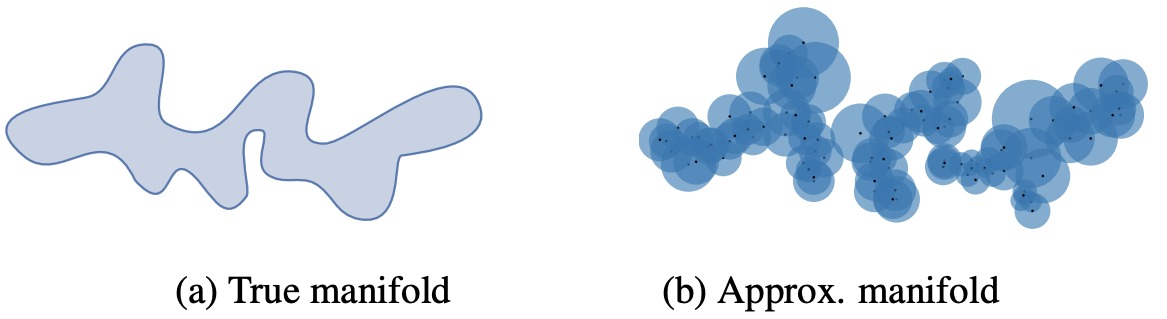
\includegraphics[width=0.7\linewidth]{figs/pr_k_nearest}
	\end{figure}
	\myfootnotewithlink{https://arxiv.org/abs/1904.06991}{Kynkäänniemi T. et al. Improved precision and recall metric for assessing generative models, 2019}
\end{frame}
%=======
\begin{frame}{Precision-Recall}
	\begin{figure}
		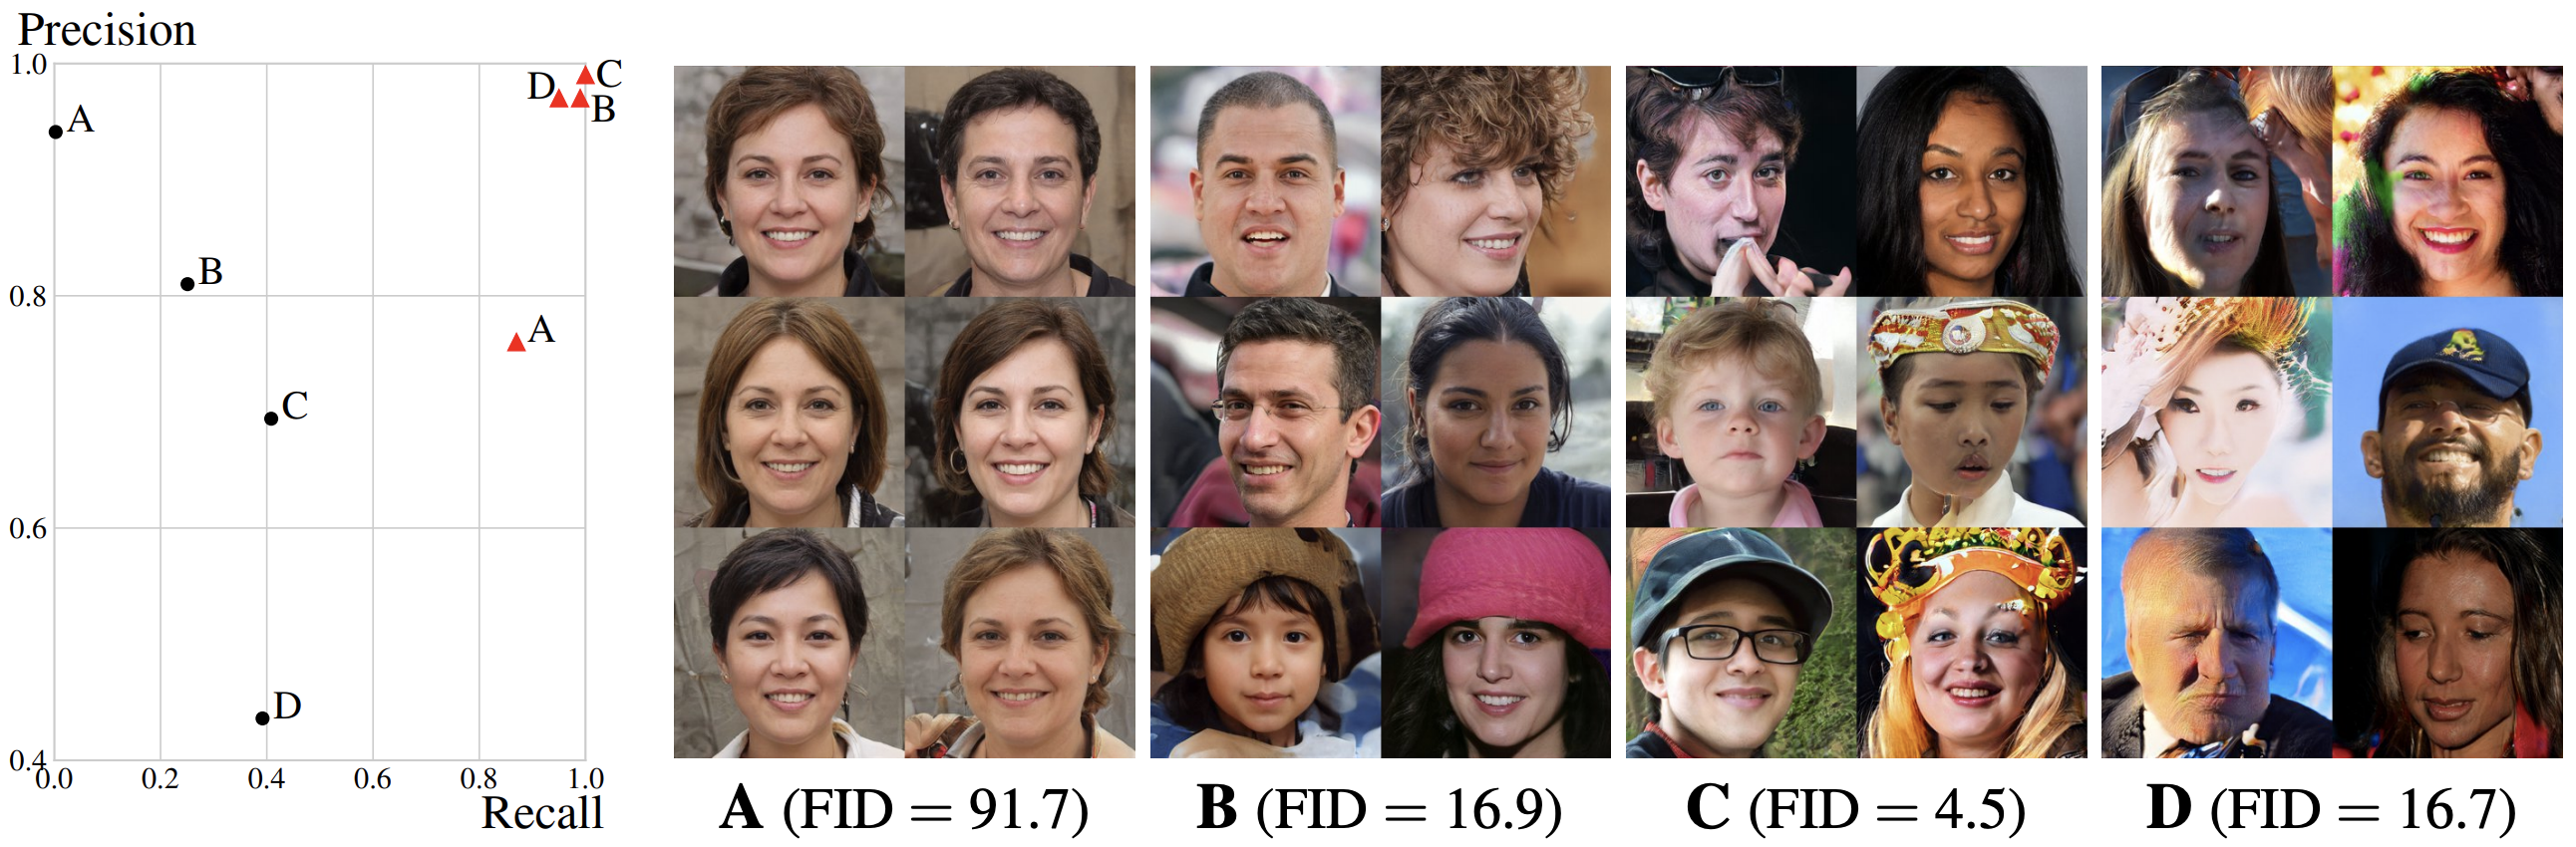
\includegraphics[width=\linewidth]{figs/pr_vs_fid}
	\end{figure}
	\begin{figure}
		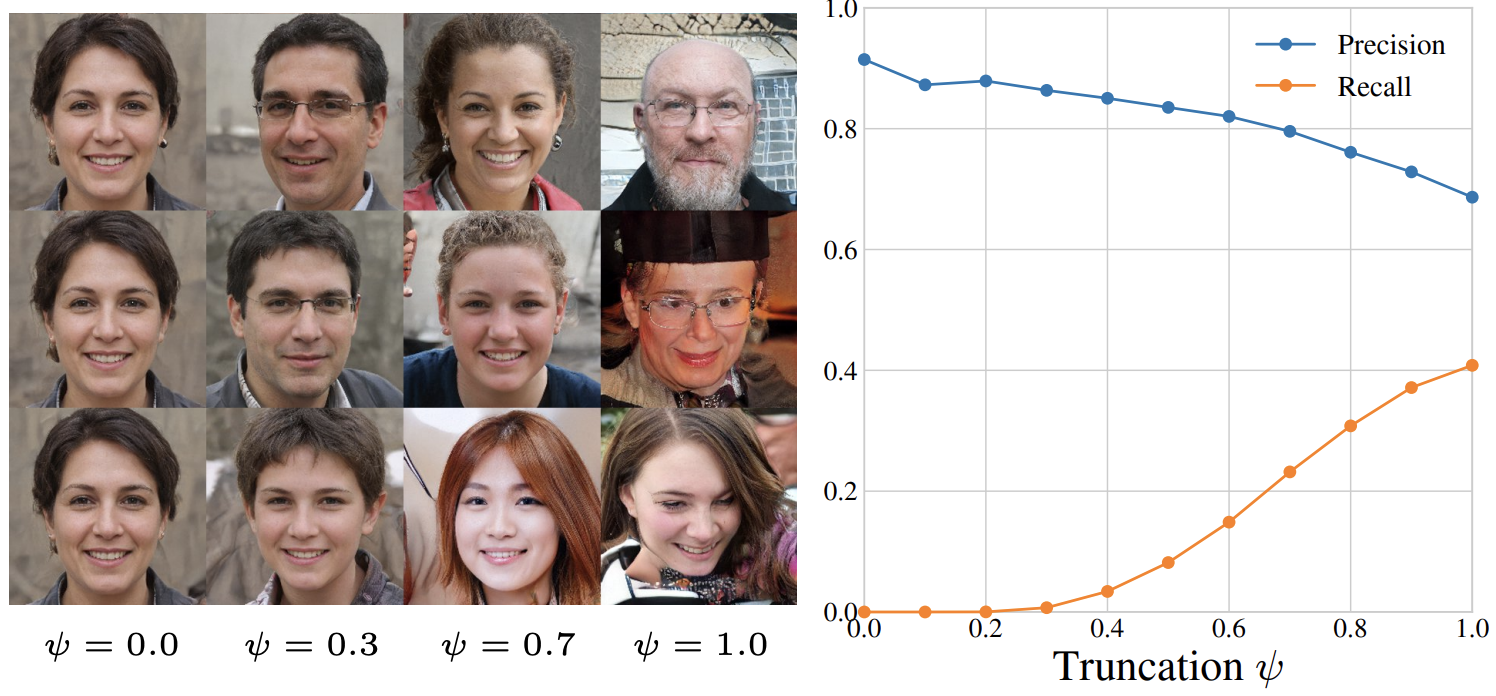
\includegraphics[width=0.75\linewidth]{figs/pr_truncation}
	\end{figure}
	\myfootnotewithlink{https://arxiv.org/abs/1904.06991}{Kynkäänniemi T. et al. Improved precision and recall metric for assessing generative models, 2019}
\end{frame}
%=======
\begin{frame}{Truncation trick}
	\begin{block}{BigGAN: truncated normal sampling}
		\vspace{-0.3cm}
		\[
			p(\bz | \psi) = \cN(\bz | 0, 1) / \int_{-\infty}^\psi \cN(\bz | 0, 1) d\bz
		\]
		Components of $\bz \sim \cN(0, \bI)$ which fall outside a predefined range are resampled.
	\end{block}
	
	\begin{block}{StyleGAN}
		\vspace{-0.2cm}
		\[
			\bz' = \hat{\bz} + \psi \cdot (\bz - \hat{\bz}), \quad \hat{\bz} = \bbE_{\bz} \bz
		\]
		\vspace{-0.2cm}
		\begin{itemize}
			\item Constant $\psi$ is a tradeoff between diversity and fidelity. 
			\item $\psi=0.7$ is used for most of the results.
		\end{itemize}
	\end{block}

	\myfootnote{\href{https://arxiv.org/abs/1809.11096}{Brock A., Donahue J., Simonyan K. Large Scale GAN Training for High Fidelity Natural Image Synthesis, 2018} \\
	\href{https://arxiv.org/abs/1812.04948}{Karras T., Laine S., Aila T. A Style-Based Generator Architecture for Generative Adversarial Networks, 2018}}
\end{frame}
%=======
\begin{frame}{Summary}
	\begin{itemize}
		\item Maximum Mean Discrepancy tries to fix some of the FID drawbacks.
		\vfill
		\item Precision-recall allow to select model that compromises the sample quality and the sample diversity.	
		\vfill 
		\item Truncation tricks help to select model with compromised samples: diverse and sharp.
	\end{itemize}
\end{frame}
%=======
\end{document} 